\documentclass{ExerciseSheet}

%Set Number of the Exercise sheet and the submission deadline.
\setExerciseSheetNumber{11}
\setSubmissionDate{xx.xx.2024}

%boolean variable to determine whether the solutions should be included
\newif\ifsolutions
\solutionstrue
%\solutionsfalse

%We have a figure in this sheet
\usepackage{graphicx}

\begin{document}


%Start with exercises
%-----------------------------------------------------------------------%

\begin{problem}
\begin{enumerate}[1.]
	\item Find all the points that satisfy the KKT conditions then solve the following constrained optimisation problem:
	    \begin{equation}\label{ConstOptI}
        \min_{(x,y)\in\mathbb{R}^2} x^2+y^2 \quad \text{subject to} \quad x\leq -1,\, y\leq -1, \, y+2x\geq 5
    \end{equation}
    \item We consider now the following problem:
		\begin{equation}\label{eq:ConstOptII}
    \max_{(x,y)\in\mathbb{R}^2} x^2+y^2 \quad \text{subject to} \quad x\geq -1,\, y\geq -1, \, y+2x\leq 5
		\end{equation}
		\begin{enumerate}[a.] 
		\item Find all the points that satisfy the KKT conditions for \eqref{eq:ConstOptII}.
    	\item Draw the feasability region $\{(x,y)\in\mathbb{R}^2:x\geq -1,\, y\geq -1, \, y+2x\leq 5\}$ and label all the points found in the previous question. Draw some level curves of the objective function $(x,y)\mapsto x^2+y^2$. Give a geometric interpretation of these points.
   	 	\item What is the solution to \eqref{eq:ConstOptII}? 
   	 	    % \footnotesize{\textbf{Note:} For this question, if your proposed solution is too long, you may explain the main steps of the proof while skipping the details of your computations.}
\normalsize
		\end{enumerate}
\end{enumerate}
\end{problem}

\ifsolutions
\vskip 0.3cm

\begin{solution}
\begin{enumerate}[1.]
	\item We are considering the problem:
	\begin{equation}\label{ConstOptI}
        \min_{(x,y)\in\mathbb{R}^2} x^2+y^2 \quad \text{subject to} \quad x\leq -1,\, y\leq -1, \, y+2x\geq 5.
    \end{equation}
	One of the requirements for $(x,y)$ to satisfy the KKT conditions is be a feasible point (i.e., to satisfy the constraints). In this case, no point is feasible since the conditions:
	\[x\leq -1,\, y\leq -1\]
	cannot hold at the same time as $y+2x\geq 5$. Consequently, there are no KKT points for the problem (\ref{ConstOptI}) and no solution. 
    \item 
    Let us put first the problem into a more familiar form, i.e., as a minimisation problem with ``negative'' constraints:
    \begin{equation}\label{ConstOptII}
    \min_{(x,y)\in\mathbb{R}^2} -x^2-y^2 \quad \text{subject to} \quad -1-x\leq 0,\, -1-y\leq 0, \, y+2x-5\leq 0
		\end{equation}
    
		\begin{enumerate}[a.] 
		\item We first write the Langrange function associated to the problem (\ref{ConstOptII}):
		\[\mathcal{L}(x,y,\alpha,\beta,\gamma)=
		-x^2-y^2
		-\alpha(1+x)
		-\beta(1+y)
		+\gamma(y+2x-5)
		\]
		The pair $(x,y)$ satisfies the KKT conditions (for this problem) if and only if there exist non-negative numbers $\alpha,\beta$ and $\gamma$ such that:
		\[
		\left\{
		\begin{array}{l}
		(x,y)\textrm { is a feasible point (i.e., satisfies the constraints.)}\\
		\nabla_{(x,y)}\mathcal{L}(x,y,\alpha,\beta,\gamma)=0\\
		\alpha(1+x)=0 ,\, \beta(1+y)=0 ,\, \gamma(y+2x-5)=0\\
		\end{array}
		\right.
		\]
		Explicitly, this reads:
		\[
		\left\{
		\begin{array}{l}
		-2x-\alpha+2\gamma=0\\
		-2y-\beta+\gamma=0\\
		\alpha(1+x)=0 ,\, \beta(1+y)=0 ,\, \gamma(y+2x-5)=0\\
		x\geq -1,\, y\geq -1, \, y+2x\leq 5\\
		\end{array}
		\right.
		\]
		We are going to separate the cases according to the manner in which the constraints at the border ($\alpha(1+x)=0$, $\beta(1+y)=0$ and $\gamma(y+2x-5)=0$) are satisfied.
		\begin{enumerate}
		\item \underline{Case 1:} $\alpha=\beta=\gamma=0$. Then $(x,y)=(0,0)$ (which is a feasible point.)
		\item \underline{Case 2:} $\alpha=\beta=0$ and $y+2x=5$. Then 
		\begin{equation}
			\begin{cases}
				y-5 +2\gamma= 0\\
				-2y+\gamma=0
			\end{cases}
		\end{equation}
		from which we get $\gamma=2$ (which is non-negative) and $(x,y)=(2,1)$.
		\item \underline{Case 3:} $\alpha=\gamma=0$ and $y=-1$. Then $x=0$ and $\beta=2$.
		\item \underline{Case 4:} $\beta=\gamma=0$ and $x=-1$. Then $y=0$ and $\alpha=2$.
		\item \underline{Case 5:} $\alpha=0$, $y=-1$ and $y+2x=5$. Then $x=3$, $\gamma=3$ and $\beta=5$.
		\item \underline{Case 6:} $\beta=0$, $x=-1$ and $y+2x=5$. Then $y=7$, $\gamma=14$ and $\alpha=30$.
		\item \underline{Case 7:} $\gamma=0$ and $x=y=-1$. Then $\alpha=\beta=2$.
		\item \underline{Case 8:} $x=y= -1$ and $y+2x= 5$. This case is impossible.
		\end{enumerate}
		To summarise, 7 points satisfy the KKT condition in the optimisation problem (\ref{ConstOptII}):
		\[(0,0),\;\;
		(2,1),\;\;
		(0,-1),\;\;
		(-1,0),\;\;
		(3,-1),\;\;
		(-1,7),\;\;
		(-1,-1)\]
    	\item 	\begin{figure}[h]
	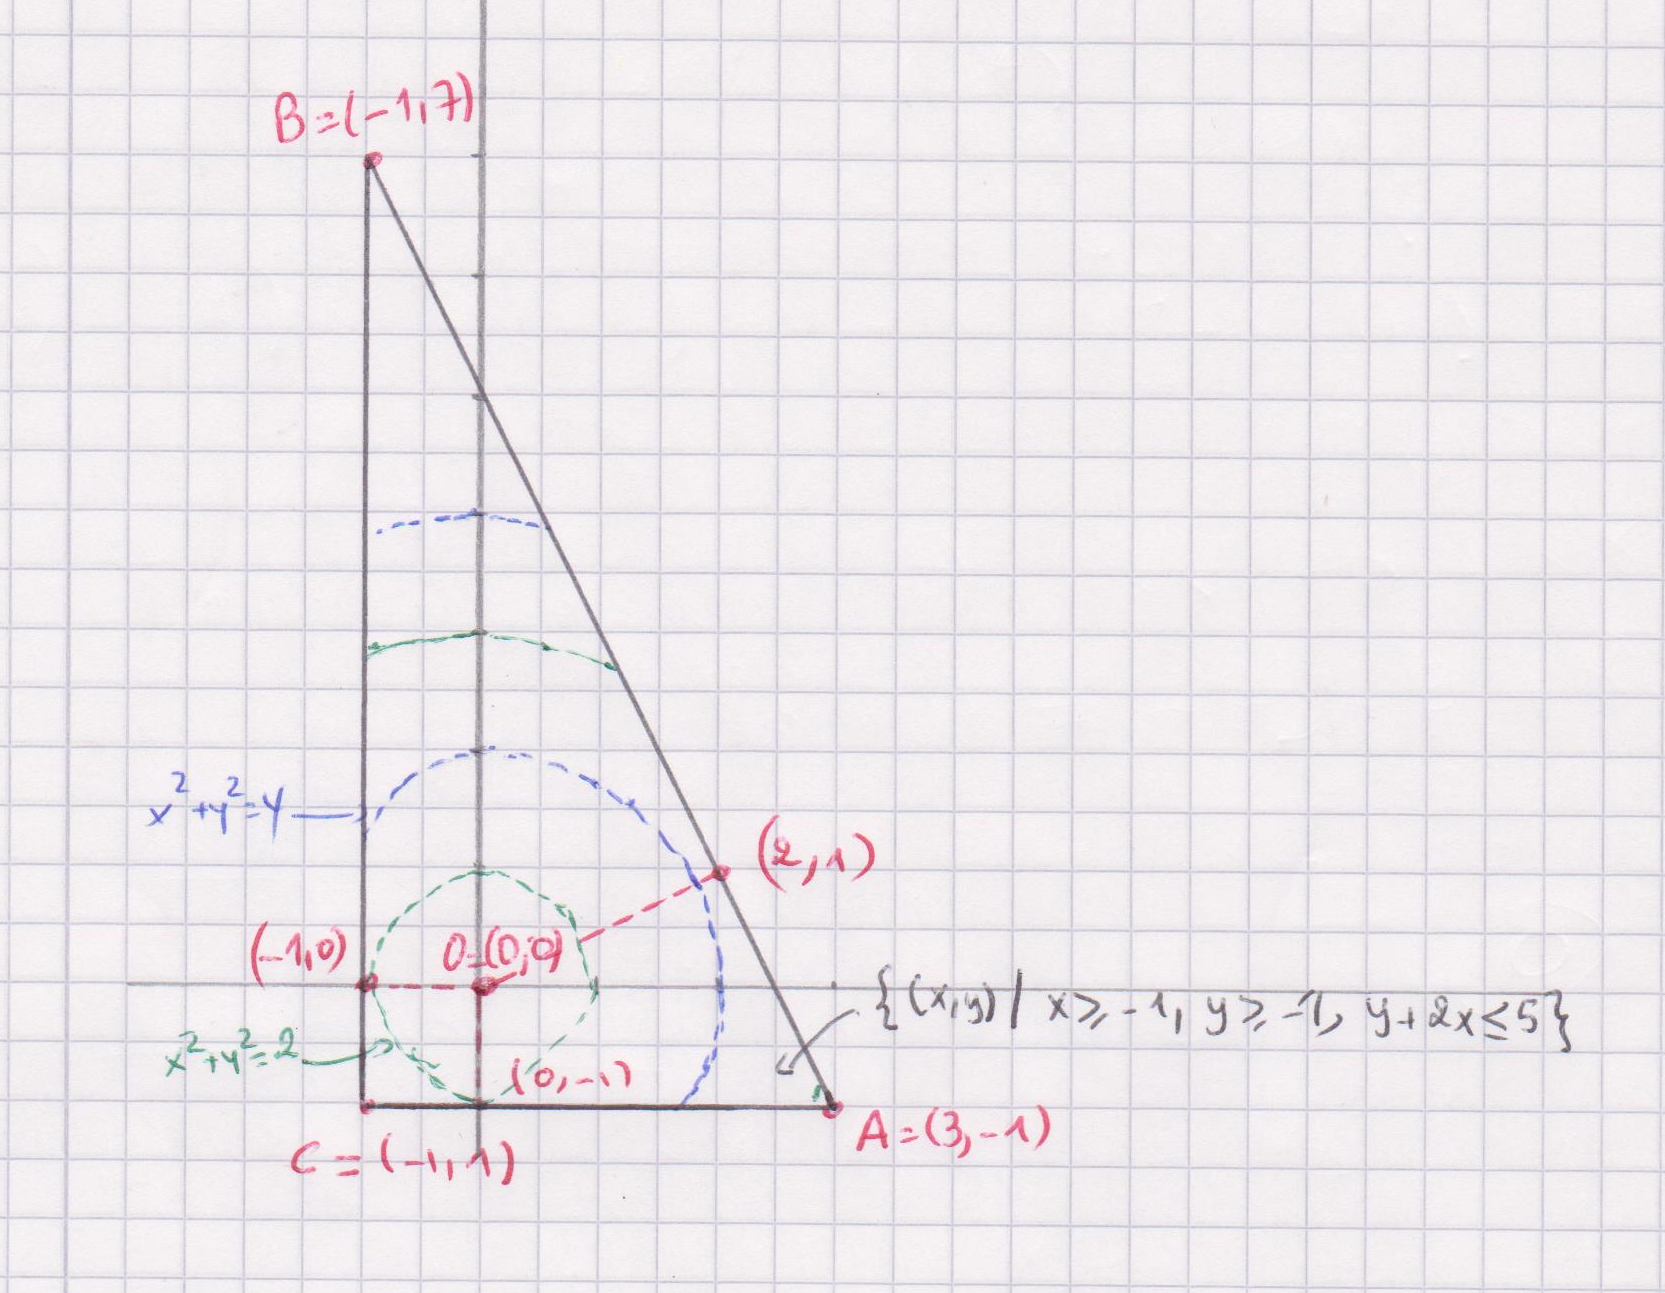
\includegraphics[scale=0.35]{ExoSheet7CurveLines}
	\centering
	\end{figure}
    	
    	
		The quantity $x^2+y^2$ measures the (square of the) distance of points in the plane from the origin $O=(0,0)$. The KKT approach has detected local extrema for this distance function in the triangle defined by the points
		\[A=(3,-1),\;\;B=(-1,7),\;\;C=(-1,-1)\] 
		 $O$ is obviously a minimiser of the quantity $x^2+y^2$. On the one hand, on each side of the triangle, the furthest points from $O$ are the vertices $A$, $B$ and $C$. On the other hand, the closest points to the origin on the edges of the triangle are the orthogonal projections of $O$ on each one of these edges. These are given by:
		 \[(2,1),\;\;
		(0,-1),\;\;
		(-1,0),\]
		which are also 3 of the stationary points of the constrained problem \eqref{eq:ConstOptII}.
		The KKT approach has detected exactly these 7 points.
   	 	\item Based either on the analytical or the geometric study above, the solution to (\ref{ConstOptII}) is one of the detected KKT points. By checking the value of the objective function for each one of these points, we conclude that (\ref{ConstOptII}) has a unique solution at the point $(-1,7)$.
		\end{enumerate}
	
\end{enumerate}

\end{solution}

\fi

%-----------------------------------------------------------------------%
\vskip 0.5cm
\begin{problem}
 Solve the following constrained optimisation problem:
			\begin{equation}\label{ConstOptIII}
    \min_{(x,y)\in\mathbb{R}^2} x-y \quad \text{subject to} \quad x^2+y^2-2\sqrt{2}x-2y\leq 1.
			\end{equation}
   It helps to proceed similarly to Problem 1, part 2. 
\end{problem}

\ifsolutions
\vskip 0.3cm

\begin{solution}
Since the objective map 
	\[(x,y)\longmapsto x-y\]
	and the constraint map 
	\[(x,y)\longmapsto x^2+y^2-2\sqrt{2}x-2y- 1\]
	are both convex and that there exist feasible points satisfying:
	\[x^2+y^2-2\sqrt{2}x-2y\leq 1\]
	(which is simply the disk of center $(\sqrt{2},1)$ and radius $2$), then finding the KKT points will give us the solution to the problem:
			\begin{equation}\label{ConstOptIII}
    \min_{(x,y)\in\mathbb{R}^2} x-y \quad \text{subject to} \quad x^2+y^2-2\sqrt{2}x-2y\leq 1.
			\end{equation}
			We start by defining the appropriate Lagrange function:
			\[\mathcal{L}(x,y,\alpha)=x-y+\alpha (x^2+y^2-2\sqrt{2}x-2y- 1).\]
			Recalling the definition of a KKT point as before, a point $(x,y)$ satisfies the KKT conditions if and only if there exists $\alpha\geq 0$ such that:
		\[
		\left\{
		\begin{array}{l}
		1+2\alpha(x-\sqrt{2})=0\\
		-1+2\alpha(y-1)=0\\
		\alpha (x^2+y^2-2\sqrt{2}x-2y- 1)=0\\
		x^2+y^2-2\sqrt{2}x-2y\leq 1\\
		\end{array}
		\right.
		\]
		The case $\alpha=0$ being impossible, then $x^2+y^2-2\sqrt{2}x-2y=1$. Using the identities
		\[x=\sqrt{2}-\frac{1}{2\alpha}\quad,\quad y=1+\frac{1}{2\alpha}\]
		we get that $\alpha=\frac{1}{2\sqrt{2}}$ then that:
		\[x=0 \quad \textrm{and} \quad y=1+\sqrt{2}.\]
		We check that this is indeed a feasible point and thus the unique solution to (\ref{ConstOptIII}).
\end{solution}

\fi

%-----------------------------------------------------------------------%
\vskip 0.5cm

\begin{exo}[On Convex Cones]
A cone is a set $S$ such that for every $x\in S$ and $\lambda \geq 0$ we have $\lambda x \in S$.

\begin{enumerate}
    \item A set $S$ is a convex cone iff the following properties hold:
    \begin{itemize}
        \item $x,y \in S \Rightarrow x+y \in S$.
        \item $x\in S, \lambda \geq 0 \Rightarrow \lambda x \in S$.
    \end{itemize}
    \item Give an example of two convex sets $S_1, S_2$ s.t. there union is not convex. 
\end{enumerate}
\end{exo}

\ifsolutions
\vskip 0.3cm
\begin{solution}
\begin{enumerate}
    \item 
\end{enumerate}
\end{solution}

\fi

%-----------------------------------------------------------------------%
\vskip 0.5cm
\begin{exo}[On Conic Hulls]
\begin{enumerate}
    \item Take any $a_1, \dots a_l \in \R^n$, then $\text{cone}(\{a_1, \dots, a_l\})$ is a closed and convex set.
     To show that the set is closed, consider the following steps:
     \begin{itemize}
         \item Show cone$(\{a_1,...,a_l\})= \bigcup_{i=1}^N cone(S_i)$, where the $S_i$ are all possible sets of linearly independent combinations of the points $a_1,...,a_l$.
         \item Show for such an $S_i$ cone$(S_i)=\{By | y\in \R^m_{\geq 0}\}$ for some suitable matrix $B$.
         \item Show each $cone(S_i)$ is closed. 
     \end{itemize}
    \item Let $S\subset \R^n$, if $S\subset T$ for some convex cone $T$, then $cone(S)\subset T$.
   
    \item Let $S=\{(x_1, x_2) | (x_1-1)^2 +x_2^2 = 1\}$, what is cone($S$)?
\end{enumerate}
\end{exo}


\ifsolutions
\vskip 0.3cm
\begin{solution}
\end{solution}
\fi

\end{document}